\chapter{Results}\label{chap:results}

In this chapter, we will introduce the results of the experiments subjecting
protein representations to various relevant perturbation regimes highlighted in
chapter \ref{chap:methods}. We first discuss the results and implications of
classical \acrshort{mmd} configurations, namely by showing how it behaves on protein
graph descriptors. We then move on to show the results of the sensitivity of the \acrshort{mmd}
values based on the underlying graph representation used to extract the various
graphs. Finally, we explore more exotic configurations of \acrshort{mmd} that we
hypothesize might be more suitable for proteins. We conclude this chapter with a
short section on the runtimes of the various elements of the computational
pipelines shown in this chapter.

\section{Overall \acrshort{mmd} behavior}

Surprisingly, we found that the behavior of \acrshort{mmd} was not as inconsistent for the
types of graphs extracted from proteins as was found on synthetic graphs by
\cite{o2021evaluation}. Figure \ref{fig:mmd_consistent_eps} exhibits a typical
trajectories of \acrshort{mmd} values as different perturbation types are progressively
added to $\varepsilon$-graphs with $\varepsilon$ set to $8$\si{\angstrom}. We
can see that both the Spearman and Pearson correlation coefficients averaged
across runs are high, indicating a high correlation between the amount of
perturbation and the normalized \acrshort{mmd} values. There is, however, an exception: the
\acrshort{mmd} obtained from the degree histogram does not behave as expected, and is very
sensitive to the addition of edges and decreases in value as more and more edges
are added. We expect that this pathology is not very common in real models and
that this can be easily detected manually.

The overall influence of the kernel on \acrshort{mmd}'s behavior subject to perturbations
such as Gaussian Noise can be seen in Figure \ref{fig:mmd_effect_kernel}. We
can see that for low values of $\sigma$ (the hyperparameter of the Gaussian
kernel, see Section \ref{sec:kernels}) and for the linear kernel, \acrshort{mmd} values
behave as desired. However, unpredictable patterns emerge when increasing
$\sigma$ and the kernel matrices can ``saturate'' quite easily. This can have
quite unpredictable behaviors: in the case of the degree histogram or the
clustering histogram, this results in an overly sensitive kernel, while the
clustering histogram remains oblivious to large amounts of perturbation.

$k$-NN graphs seem to behave similarly to $\varepsilon$-graphs, in that they are
able to detect perturbations - see Figure \ref{fig:mmd_k_nn_graphs} for an
example with 2-NN graphs. However, they are extremely sensitive to Gaussian
noise and to the addition of edges (see the upper left and the upper mid pane of Figure
\ref{fig:mmd_k_nn_graphs}). Presumably, this is because very small amounts of
noise ($<4$\si{\angstrom}) affect the direct local neighborhood of each node
very significantly in such a way that the resulting $k$-NN graph is rapidly
disrupted, which is not necessarily the case with other perturbations. We note
that overall the $\varepsilon$-graphs behave more consistently than $k$-NN
graphs, with 13 out of 21 Pearson's correlation coefficients being higher in
$\varepsilon$-graphs compared to $k$-NN graphs and 11 out of 21 Spearman's
correlation coefficients being higher in 8\si{\angstrom}-graphs compared to 2-NN
graphs. Even when the $\varepsilon$-graphs did not compare favorably, it was by
a considerably lower margin than $k$-NN graphs in a similar setting. This effect
seems to be mitigated by increasing $k$, but this comes at the cost of a lower
Spearman correlation coefficient, which is even less desirable - see Figure
\ref{fig:k_vs_turbulence_gaussian_noise}. Changing kernel parameters did not
alleviate the pathologies (see Supplementary Figure
\ref{fig:mmd_effect_kernel_knn}) and had the same overall effect as observed in
Figure \ref{fig:mmd_effect_kernel}. We, therefore, proceed with further analysis
using $\varepsilon$-graphs.


\begin{figure}
  \centering
  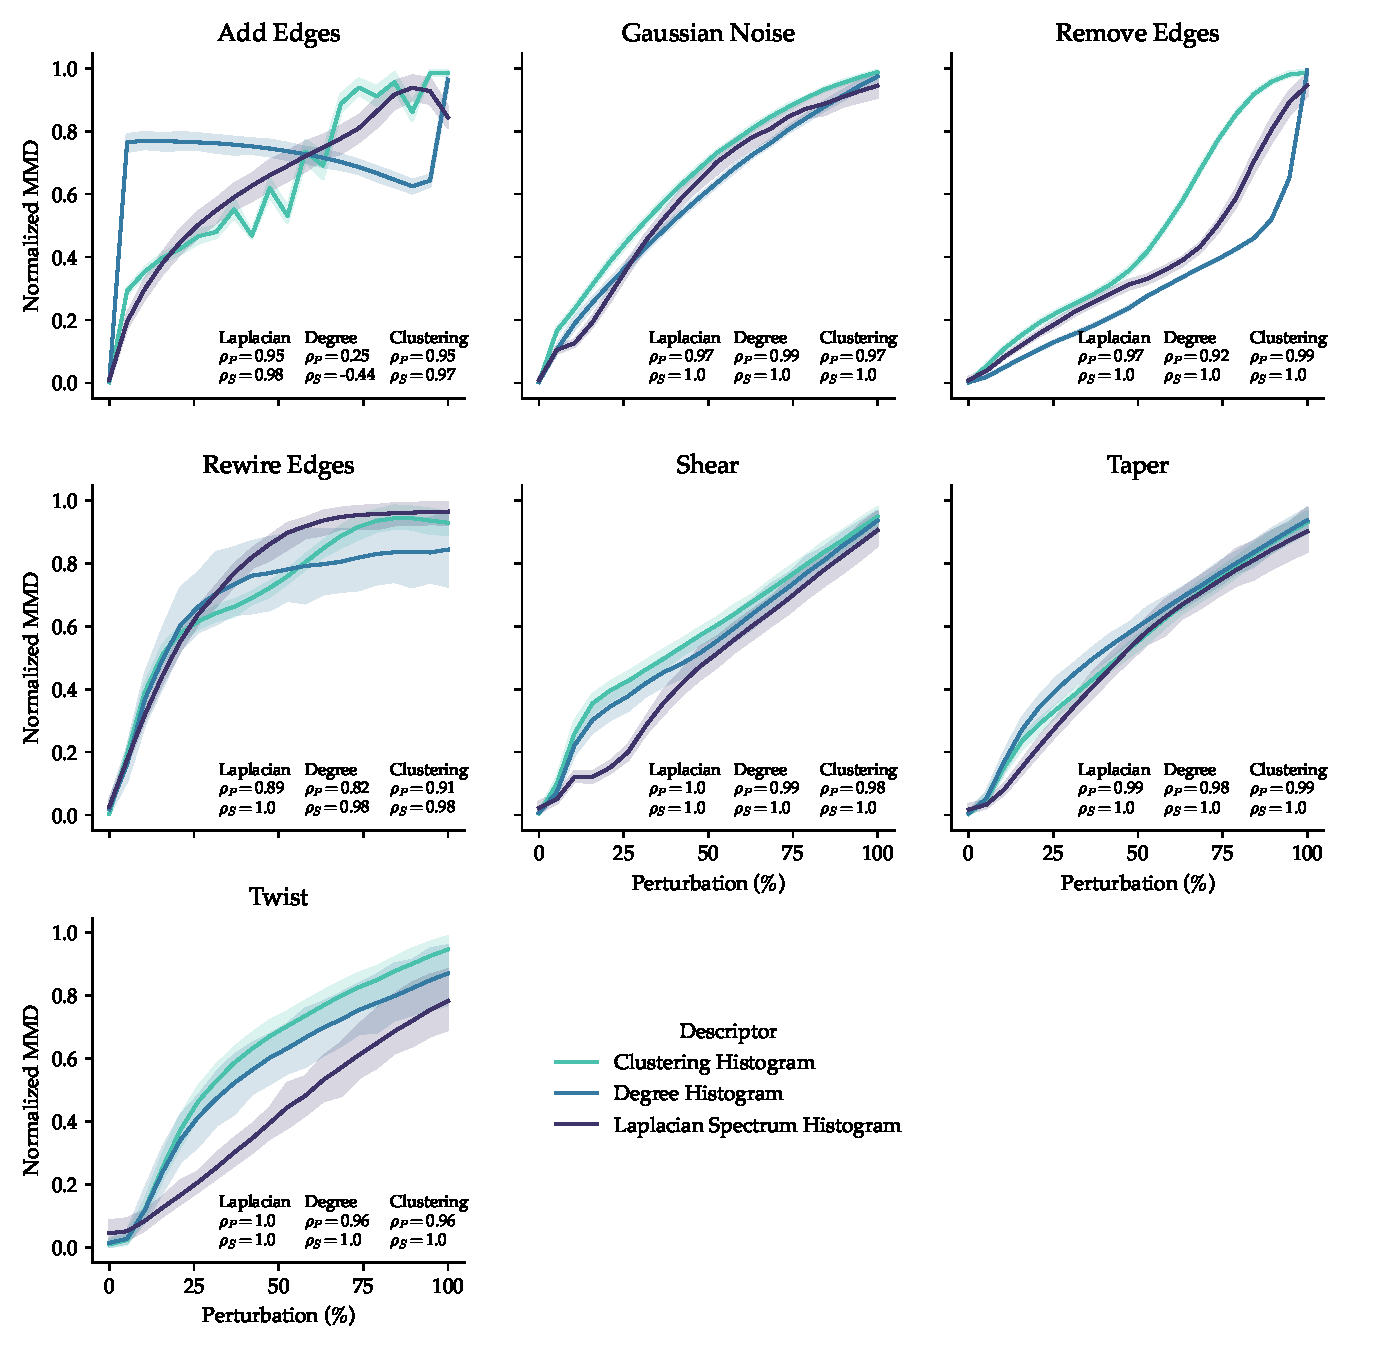
\includegraphics[width=\textwidth]{./figures/results/res_1_1.pdf}
  \caption[Overall behaviour of \acrshort{mmd} using graph-based descriptors.]{\acrshort{mmd} vs.
perturbation (in \%) for various graph descriptors of the 8\si{\angstrom}-graphs
under different perturbations regimes. The kernel used to obtain these graphs is
the RBF Kernel with bandwidth 0.01. $\rho_{S}$: average Spearman correlation
coefficient across runs. $\rho_{P}$: average Pearson correlation coefficient
across runs. Save for the degree histogram behaviour when edges are added, we
see that most \acrshort{mmd} configurations behave well, i.e. there is a high correlation
betweeen the \acrshort{mmd} values and the perturbation.}
  \label{fig:mmd_consistent_eps}
\end{figure}


\begin{figure}
  \centering
  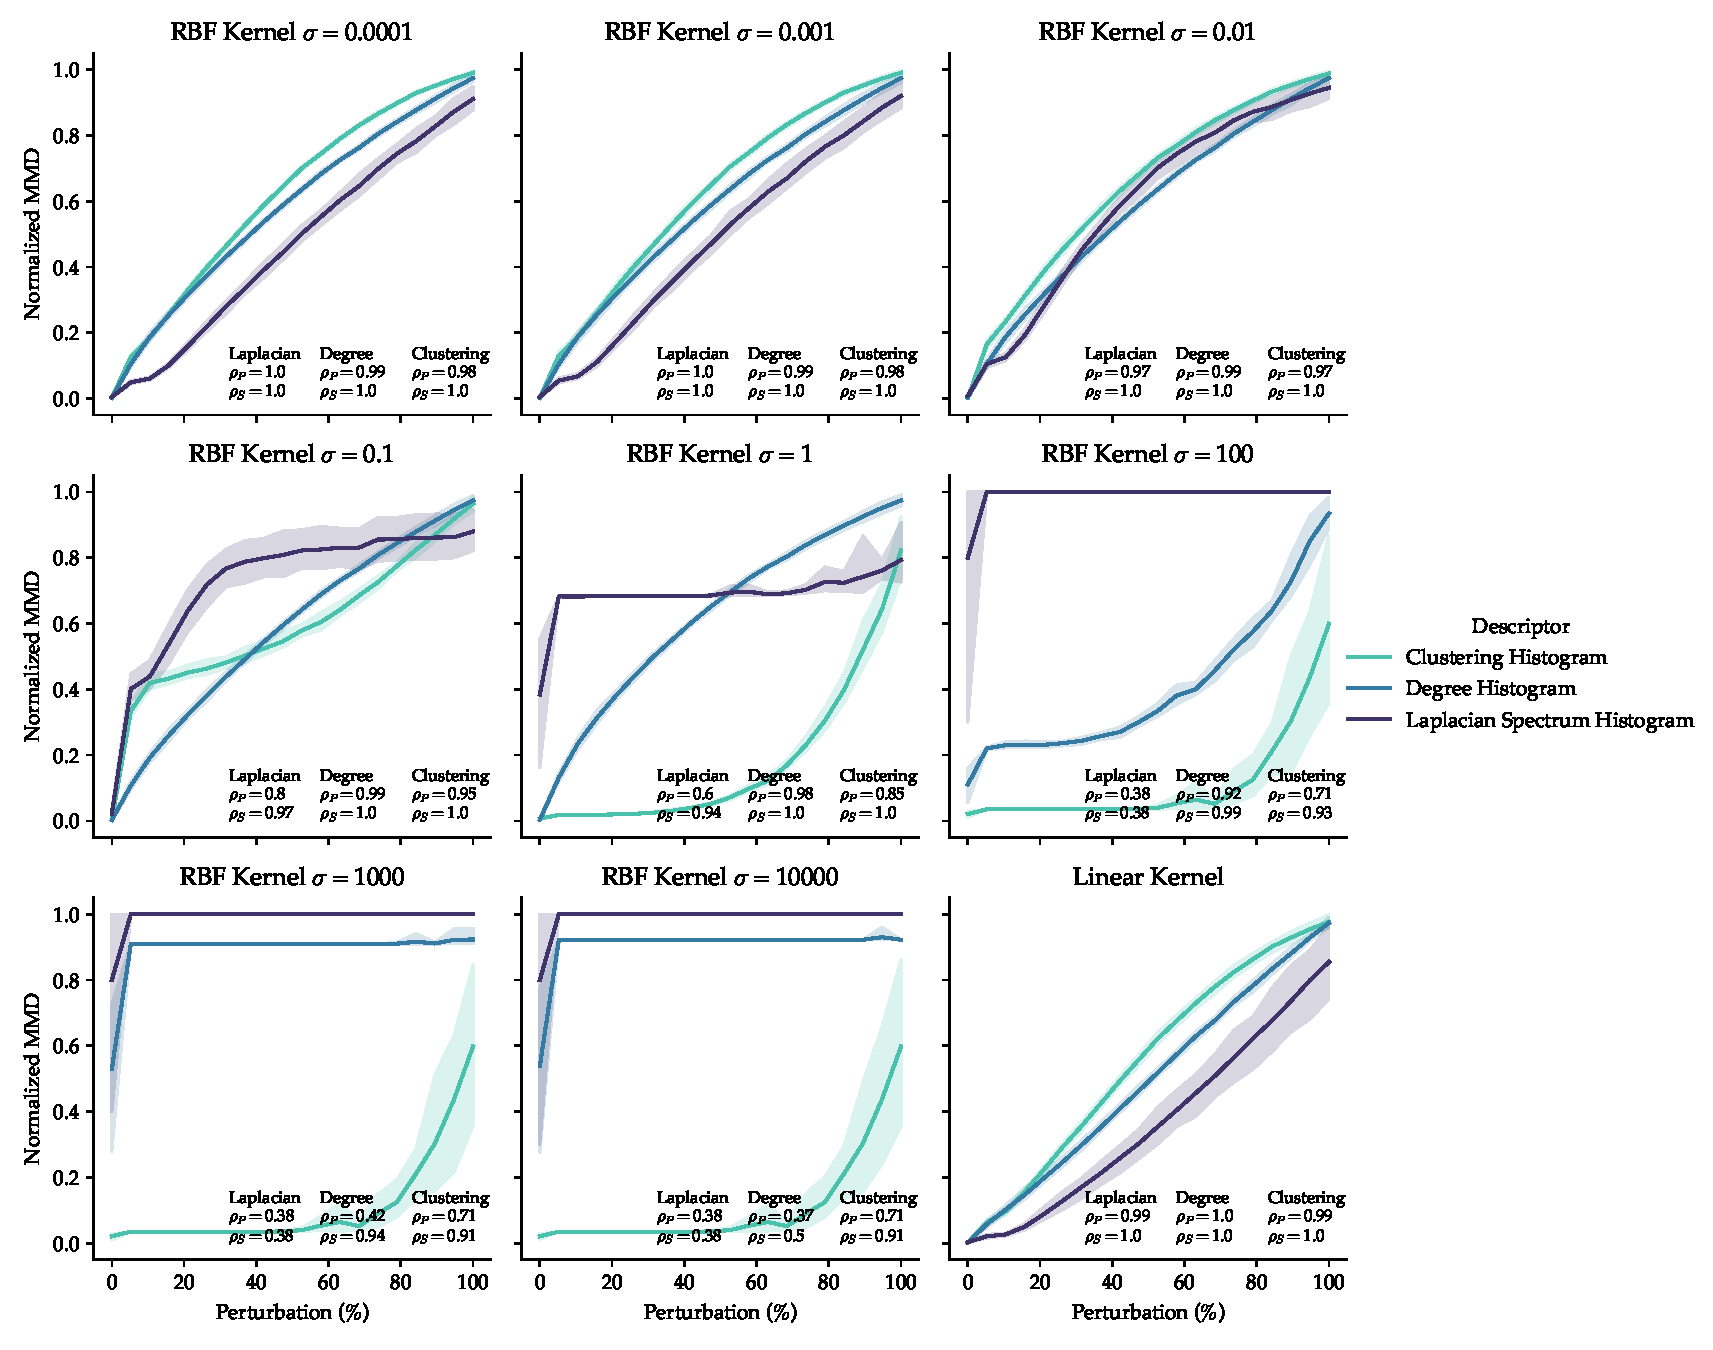
\includegraphics[width=\textwidth]{./figures/results/res_1_2.pdf}
  \caption[Influence of kernel parameters on \acrshort{mmd} behaviour.]{\acrshort{mmd} vs. Gaussian
noise perturbation (in \%) for various graph descriptors of the
8\si{\angstrom}-graphs. $\rho_{S}$: average Spearman correlation coefficient
across runs. $\rho_{P}$: average Pearson correlation coefficient across runs.
The kernel here is shown on top of each subplots. We can see that reasonable
behaviour of the RBF kernel can be seen when $\sigma<1$. The linear kernel also
behaves well.}
  \label{fig:mmd_effect_kernel}
\end{figure}

\begin{figure}
  \centering
  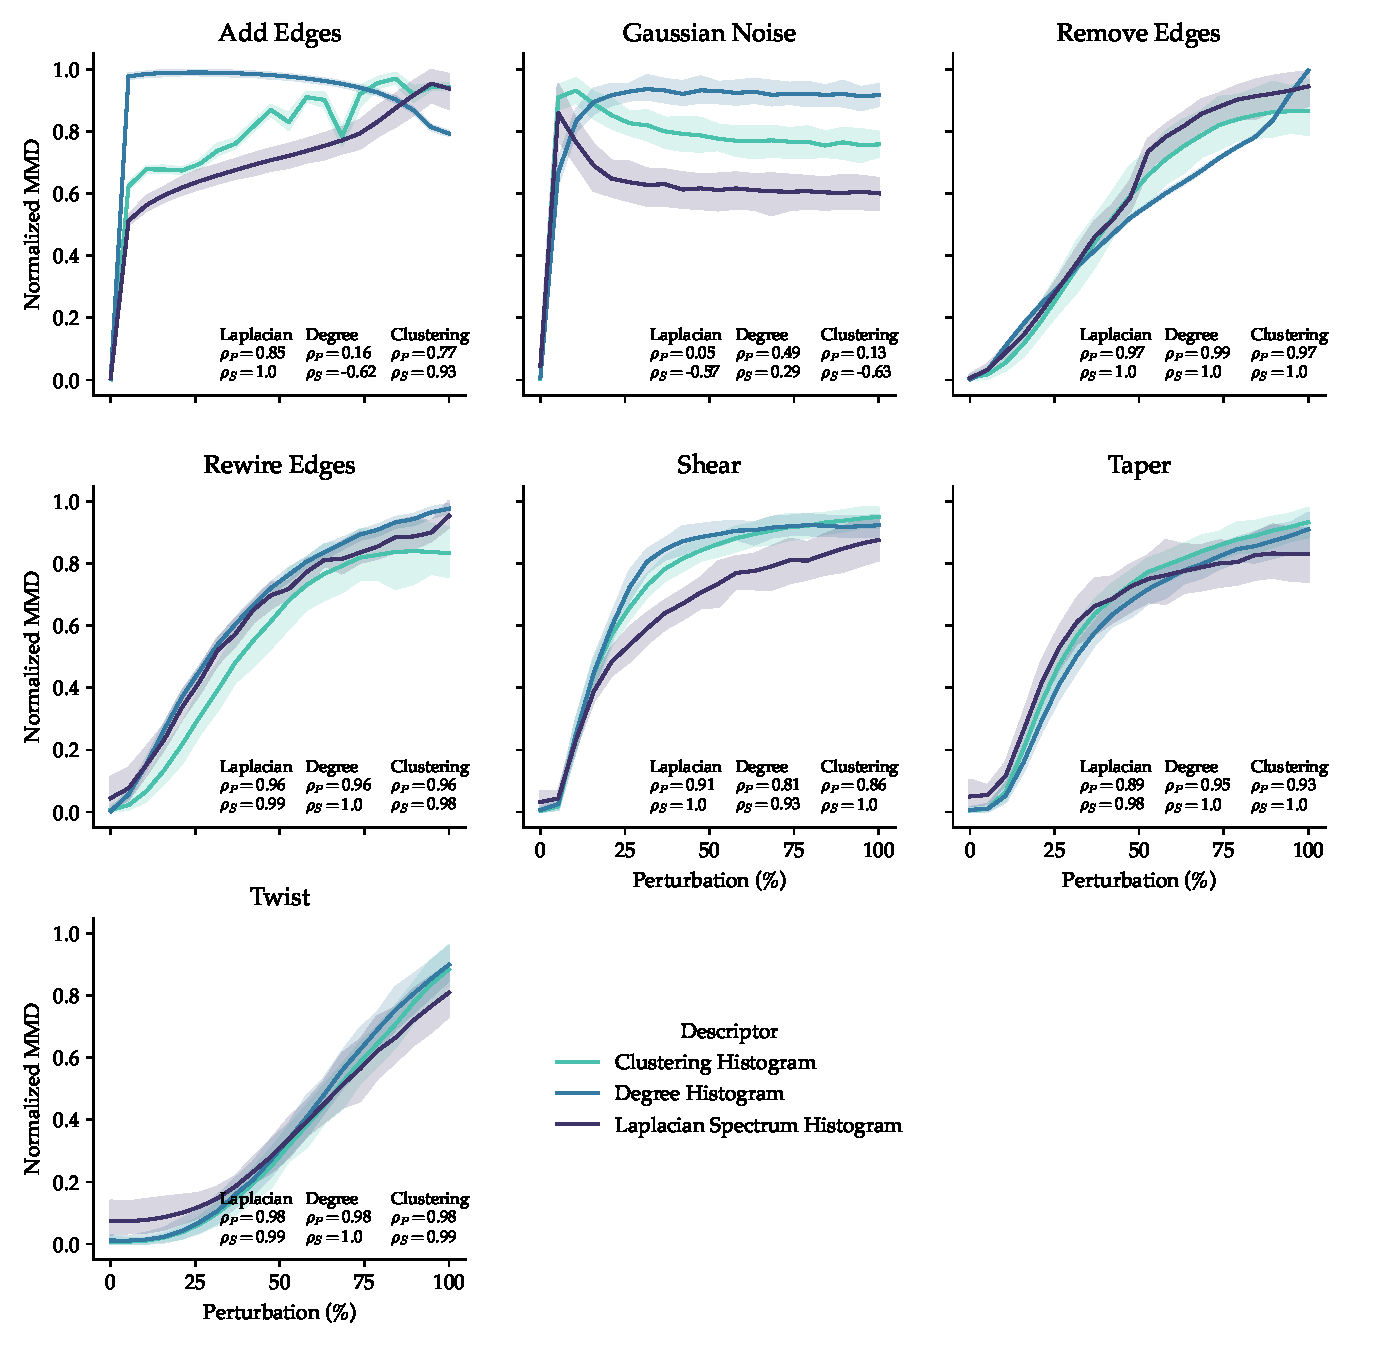
\includegraphics[width=\textwidth]{./figures/results/res_1_3.pdf}
  \caption[2-nearest-neighbour graphs result in descriptors highly sensitive to
the addition of edges and Gaussian noise.]{\acrshort{mmd} vs. Gaussian noise perturbation
(in \%) for various graph descriptors of the 2-nearest-neighbour graphs.
$\rho_{S}$: average Spearman correlation coefficient across runs. $\rho_{P}$:
average Pearson correlation coefficient across runs. We can see that this
particular representation results in \acrshort{mmd} values that are very sensitive to the
addition of edges or Gaussian noise, regardless of the descriptor used.}
  \label{fig:mmd_k_nn_graphs}
\end{figure}

\begin{figure}
  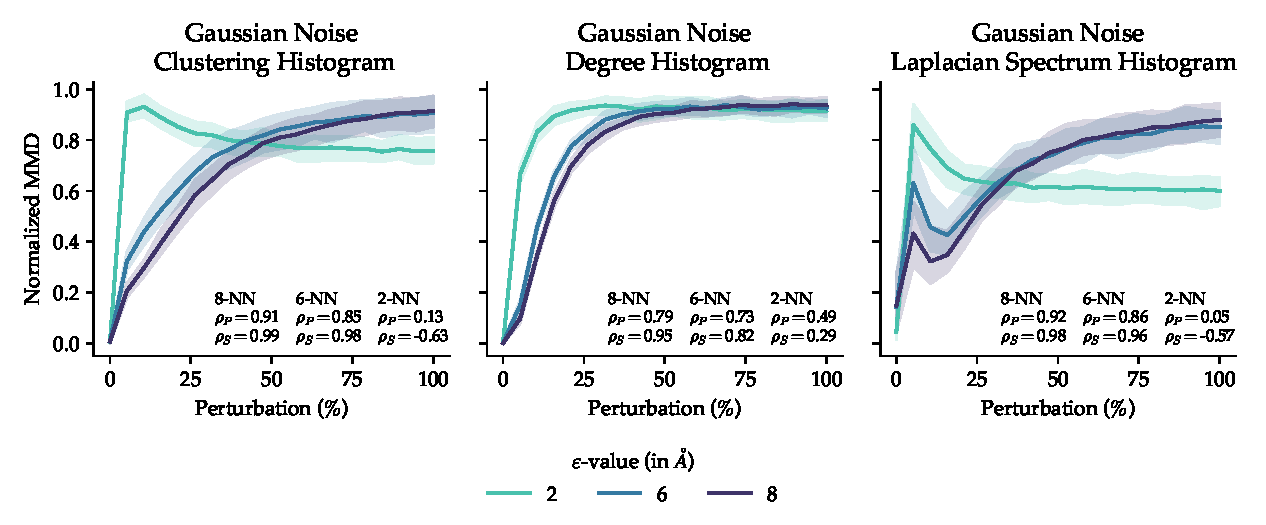
\includegraphics[width=\textwidth]{./figures/results/res_1_4.pdf}
  \caption[Influence of $k$ on the resulting \acrshort{mmd} values.]{\acrshort{mmd} vs. Gaussian noise
perturbation (in \%) for various graph descriptors and values of $k$ used to
extract the $k$-NN graph. $\rho_{S}$: average Spearman correlation
coefficient across runs. $\rho_{P}$: average Pearson correlation coefficient
across runs. Overall, the smaller the $k$, the more sensitive the
\acrshort{mmd}. Choosing $k=2$ results in sometimes unpredictable behaviour depending on
the descriptor chosen (like the clustering and laplacian spectrum histograms).}
  \label{fig:k_vs_turbulence_gaussian_noise}

\end{figure}

% \acrshort{mmd} is quite stable, somewhat contradicts what obray is saying. Maybe due to
% the different nature of the graphs.

\section{Influence of the graph representation on the sensitivity to perturbations}\label{sec:results_sensitivity}

In the last section, we discussed the notion of sensitivity of a particular \acrshort{mmd}
configuration to perturbations. We explore this idea further here. Specifically,
we investigate the impact of the $\varepsilon$ threshold on the resulting
sensitivity of the \acrshort{mmd} configuration to various perturbations affecting the
underlying point cloud. Figure \ref{fig:mmd_sensitivity_eps} shows that, in
general, the lower the $\varepsilon$, the more sensitive the \acrshort{mmd} to
perturbations. Low sensitivity to perturbation might be useful in the early
stages of modeling when generated samples only need to \emph{coarsely} match
the reference samples. Conversely, a higher sensitivity to perturbations might
be useful when trying to \emph{finely} distinguish a set of anomalous samples
from the reference samples. Additionally, we can see that under the Gaussian
noise, twisting and tapering perturbation, larger values of $\varepsilon$
introduce larger variations in \acrshort{mmd} values.

\begin{figure}
  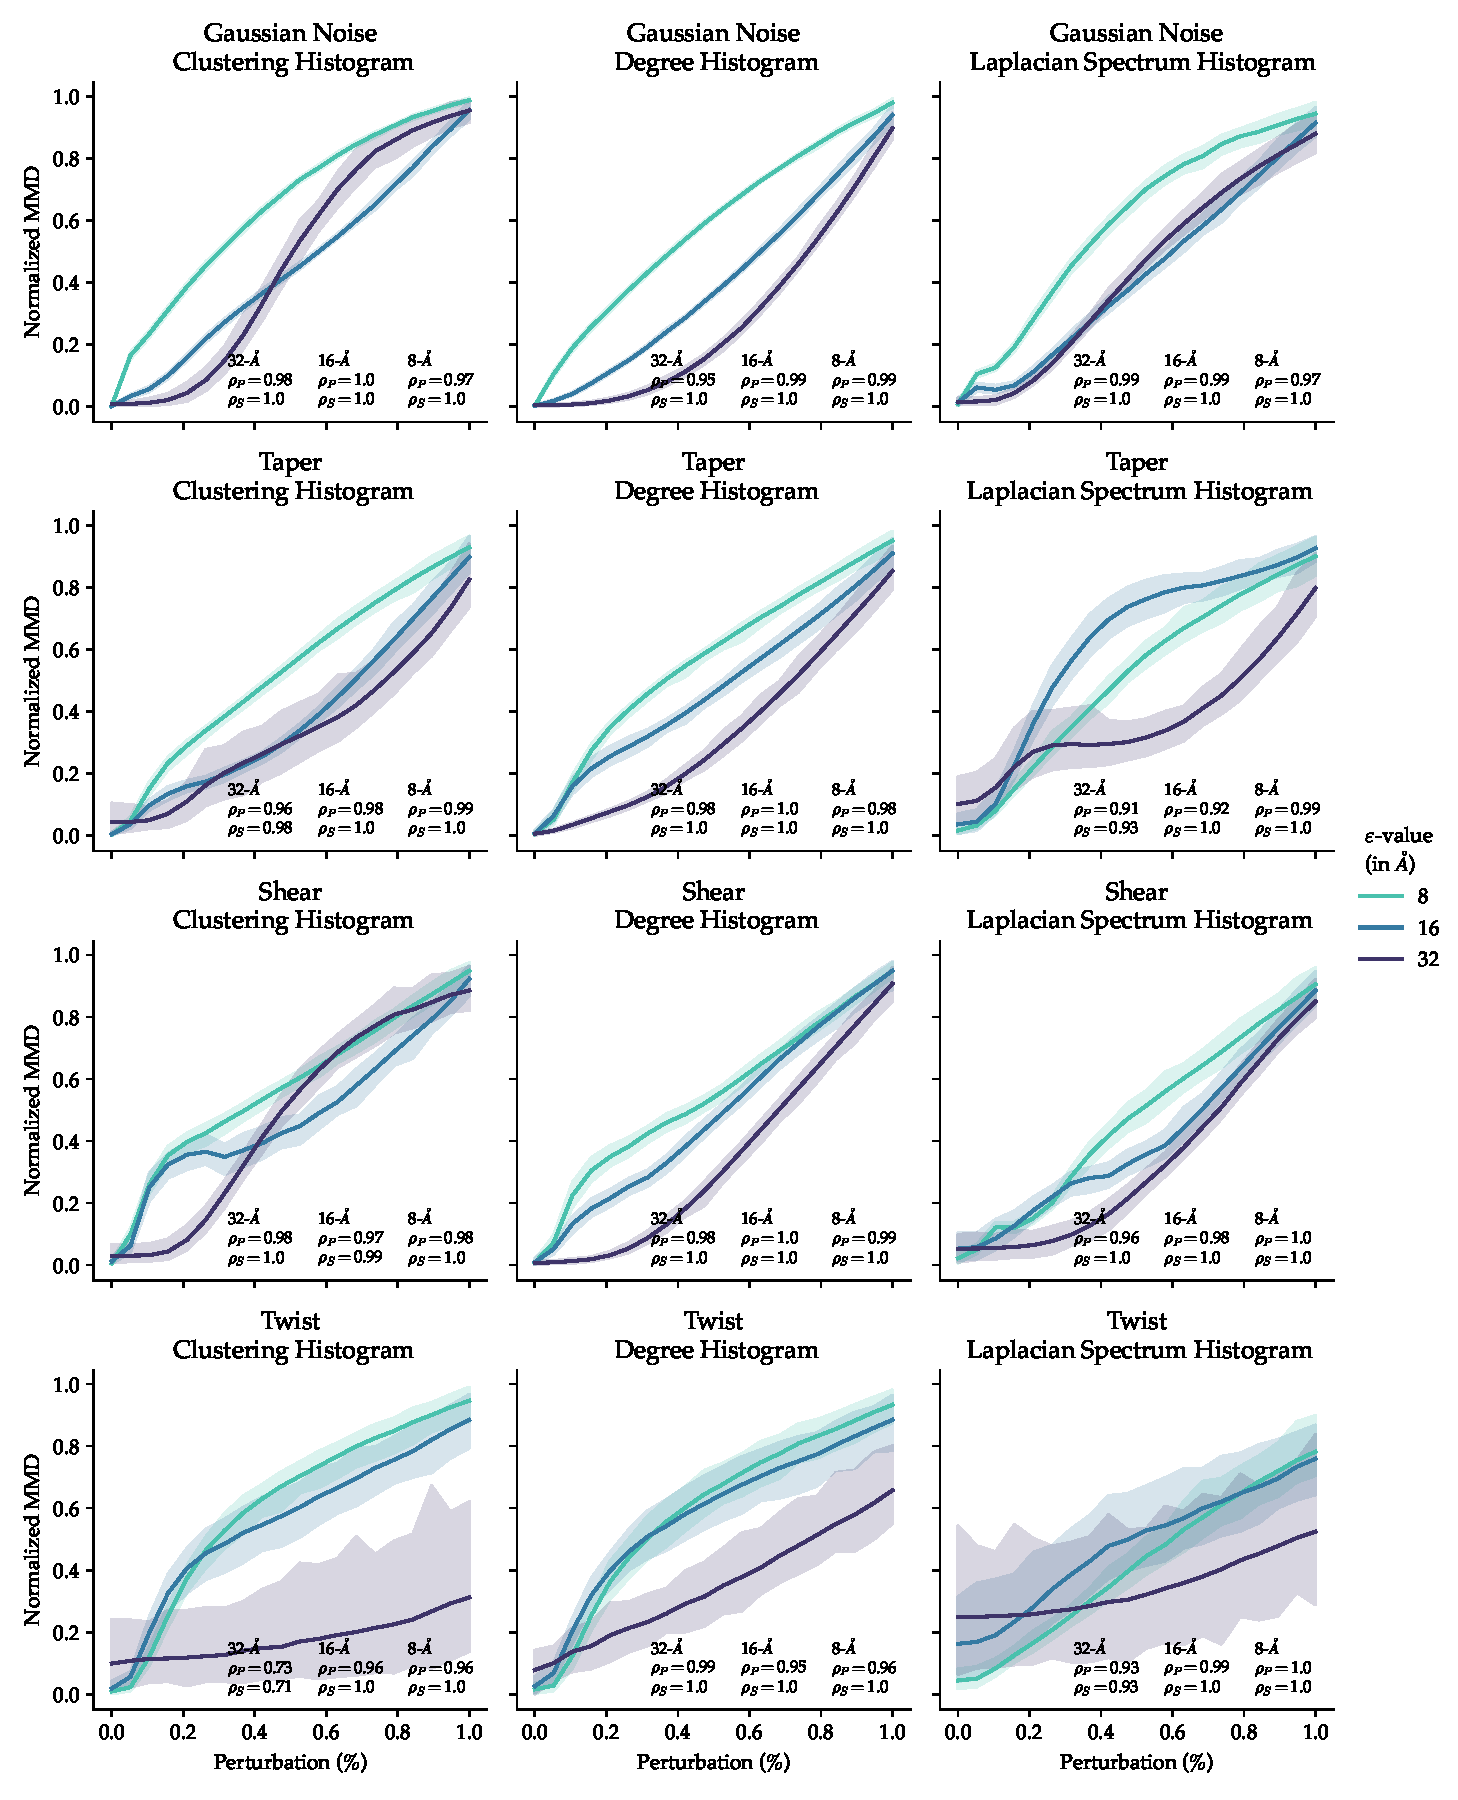
\includegraphics[width=\textwidth]{./figures/results/res_2_1.pdf}
  \caption[Influence of $\varepsilon$ on the sensitivity of \acrshort{mmd} to perturbations.]{\acrshort{mmd} vs. point cloud perturbation for various descriptors. In general,
when graphs are extracted with a lower $\varepsilon$ value, the \acrshort{mmd} curve
increases more rapidly. The only exception to this trend is the laplacian
spectrum histogram descriptor under the tapering perturbation.}
  \label{fig:mmd_sensitivity_eps}
\end{figure}

\section{Graph Kernels}\label{sec:results_graph_kernels}
% TODO compare WL with ESM (no modelling bias for WL on paper, might be a
% weakness since some mutations might not have a functional effect.)

The results of the behavior of the Weisfeiler-Lehman kernel (see Sections
\ref{sec:kernels} and \ref{sec:methods_kernels}) can be seen in Figure
\ref{fig:wlk}. Contrary to the tendencies observed in Section
\ref{sec:results_sensitivity}, \acrshort{mmd}s obtained using the Weisfeiler-Lehmann
kernels on 8\si{\angstrom} graphs are very insensitive to medium levels of perturbations,
and even completely oblivious to rewiring of graphs and generally insensitive to
graph perturbations unless highly perturbed (see upper row of Figure \ref{fig:wlk}). The most likely explanation
is that the diversity of Weisfeiler-Lehman hashes (i.e. neighborhoods) observed within perturbed or
unperturbed samples is relatively high, which makes distinguishing between the
two a high threshold to overcome. This drawback could disappear if one is working on
a more targeted set of morphologically similar proteins with a lower diversity
of Weisfeiler-Lehman hashes, but this is beyond the scope of the thesis.

\begin{figure}
  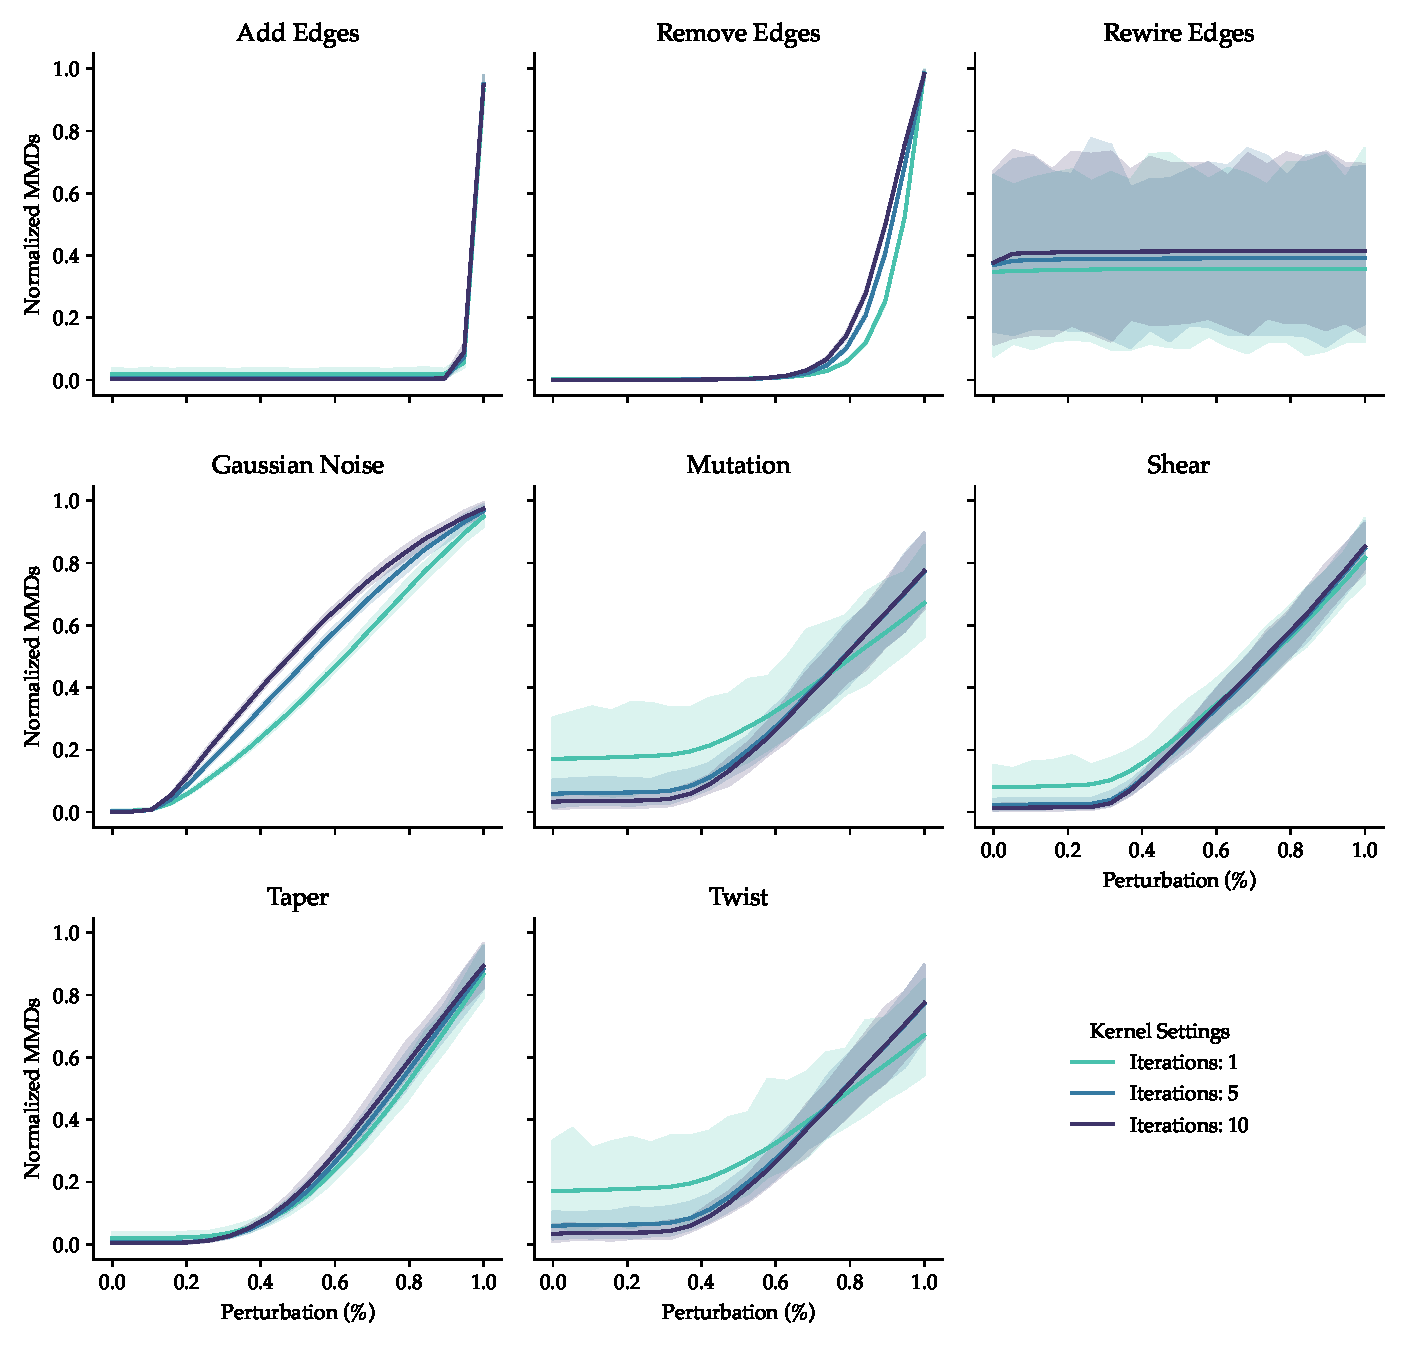
\includegraphics[width=\textwidth]{./figures/results/res_3.pdf}
  \caption[Normalized \acrshort{mmd} values using the Weisfeiler-Lehman kernel subject to
  various perturbations.]{\acrshort{mmd} vs.
perturbations using the Weisfeiler-Lehman kernel using the
8\si{\angstrom}-graphs as inputs. We see that high levels of perturbations are
required to raise the normalized \acrshort{mmd} values. We also see that \acrshort{mmd}s computed with
the Weisfeiler-Lehman kernel are insensitive to the rewiring of edges, and
results in \acrshort{mmd}s with a high inter-run variance.}
  \label{fig:wlk}
\end{figure}

\section{Protein-specific descriptors}\label{sec:results_protein_descriptors}

The behaviour of \acrshort{mmd} values derived from the protein-specific descriptor
functions described in section \ref{sec:descriptors} are shown in Figure
\ref{fig:protein_specific_descriptors}. The dihedral angles descriptor is
extremely sensitive to any kind of Gaussian noise and even decreases in value
when the kernel is not parametrized properly when increasing the shearing. This
is overall a good sign, as it will flag proteins that are unrealistic. The
interatomic distance histogram also behaves well. However, it shows high
variance when twisting the protein, presumably because the intra-sample variance
in distances is a threshold hard to overcome. This phenomenon can also be
noticed in Figure \ref{fig:wlk} with the Weisfeiler-Lehman kernel and could
disappear when working on morphologically similar proteins as highlighted in
Section \ref{sec:results_graph_kernels}. Another attractive aspect of this class
of descriptors is that they are very cheap to compute -- see further results in
Section \ref{sec:results_runtime}.

\begin{figure}
  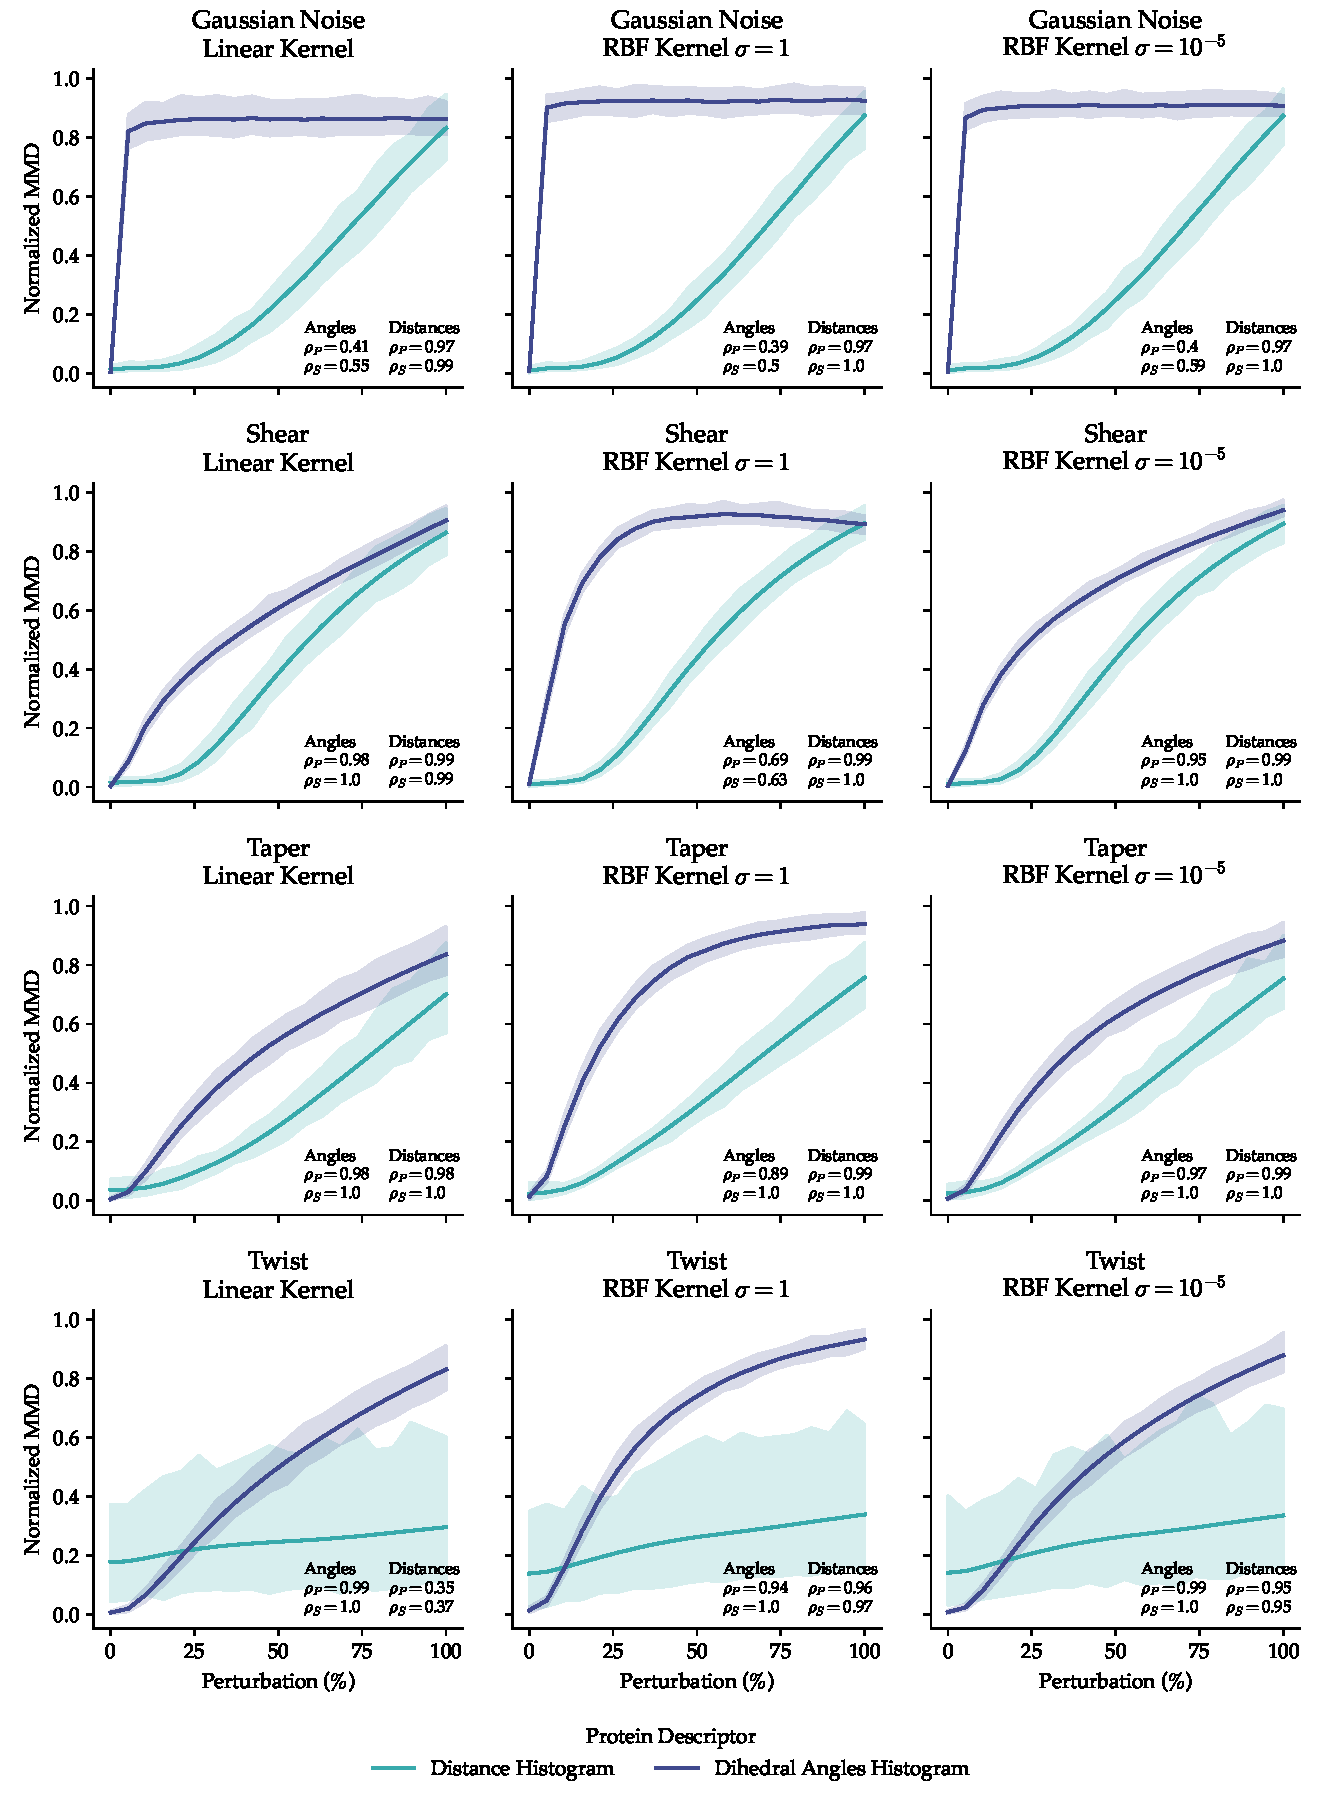
\includegraphics[width=\textwidth]{./figures/results/res_4.pdf}
  \caption[\acrshort{mmd} vs. perturbations using the two novel protein descriptors.]{\acrshort{mmd}
vs. perturbations (in \%) using the two novel protein descriptors shown in Section
\ref{sec:descriptors}. Various kernel configurations are shown here. Those
descriptors behave very well overall, with the dihedral angles descriptors being
especially sensitive to Gaussian noise. The distance histogram exhibits
particularly higher inter-run variance especially when subject to twisting
pertubations.}
  \label{fig:protein_specific_descriptors}
\end{figure}

\section{\acrshort{mmd} From Learned Embeddings}

Because the only constraint of the input vectors to the kernels accepting
fixed-length vectors as inputs is that they are in $\R^d$, we can input
fixed-length vector embeddings into them, leveraging the immense progress made
in the past decade regarding embeddings of structured data, specifically protein
sequences as highlighted in Section \ref{sec:mmd}. The only perturbation such a
learned embedding would be sensitive to is changes in the protein sequence. As
such, we investigated how the \acrshort{mmd} values increase with increasing point mutation
probabilities with various kernels, as seen in Figure \ref{fig:esm_descriptor}.
We find that the kernel used does not have any bearing on the \acrshort{mmd} behavior as
long as $\sigma<1$ for the RBF kernel. Overall, we see that even in these low
mutation regimes, the \acrshort{esm} embedding is sensitive enough to detect such changes.
More sequence-specific perturbations are required to assess the
applicability of the \acrshort{esm} embedding as a sequence descriptor, such as
translocation of subsequences, additions, deletions, etc. However, the early
results of such a descriptor shown in this thesis are promising

\begin{figure}
  \centering
  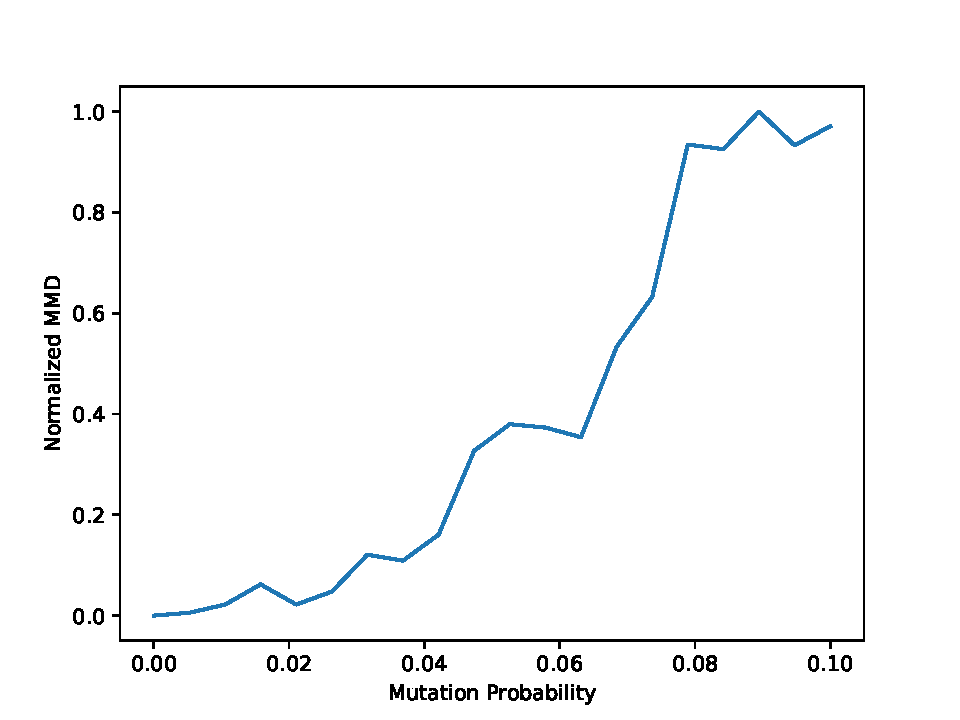
\includegraphics[width=\textwidth]{./figures/results/res_5.pdf}
  \caption[\acrshort{mmd} using \acrshort{esm} embeddings.]{\acrshort{mmd} vs. mutation probability using the \acrshort{esm}
learned embeddings with various kernels. The correlation coefficients of the
resulting \acrshort{mmd}s with RBF kernels with $\sigma<1$ and the linear kernel are high,
therefore making them good configurations for sequences. This analysis should be
complemented by complementary sequence-specific perturbations -- see Section
\ref{sec:discussion_realistic_proteins} for details.}
  \label{fig:esm_descriptor}
\end{figure}


\section{Topological Descriptors And Kernels}\label{sec:results_topo_kernels}

Figure \ref{fig:tda_kernels} shows the behavior of both the multi-scale kernel
and persistence Fisher kernel. Overall, we can see that they are among the best
performing metrics in this thesis, with high correlations and low inter-run
variation. While they cannot detect changes in node labels in the current
setting, hence not being able to detect mutations, we will show in Section
\ref{sec:tda_limitations} how this could be alleviated. For computational
reasons, we did not compute variations of different kernel parameters, although
one could speed up the operation by precomputing the kernel matrices, and only
later multiplying the matrix by different constants (see Appendix A.5 of
\cite{o2021evaluation}).

\begin{figure}
  \centering
  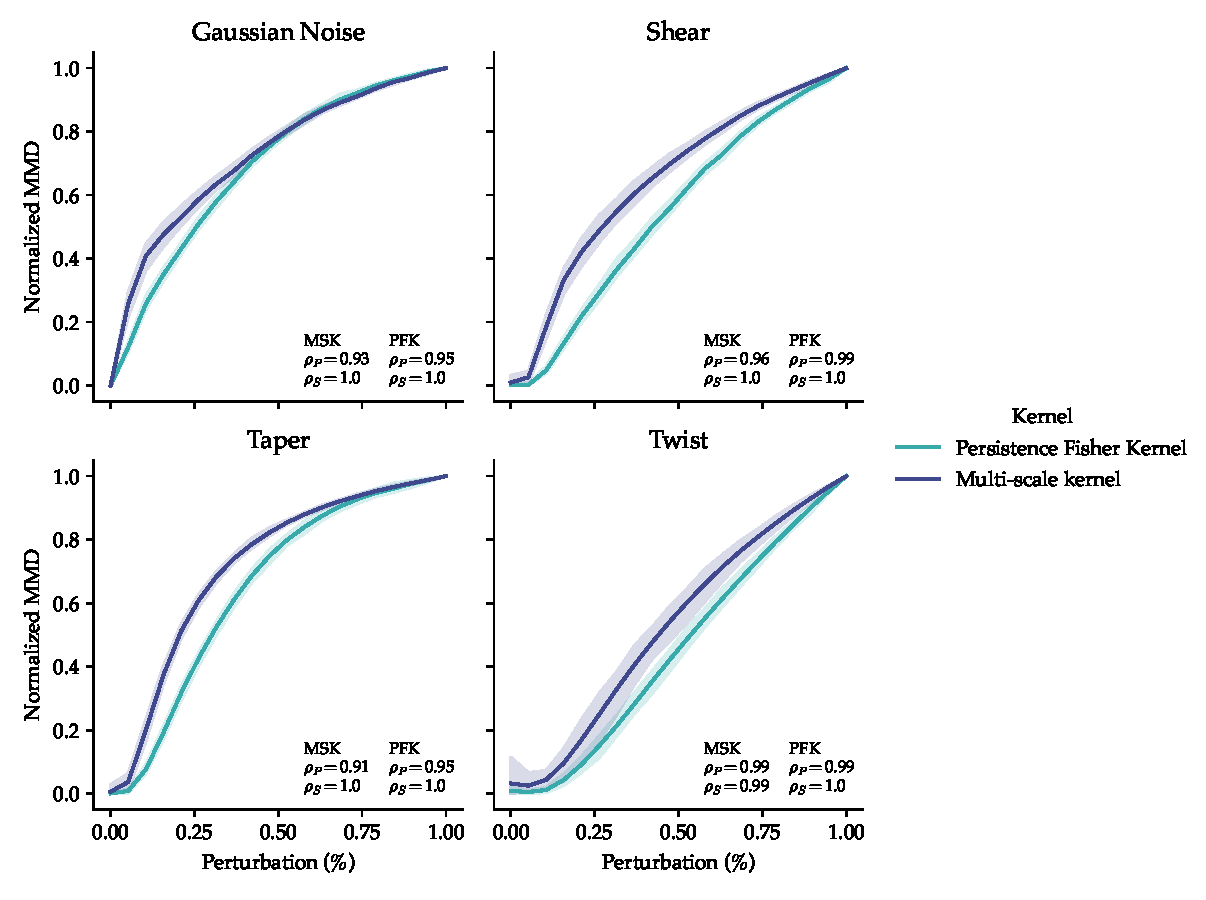
\includegraphics[width=\textwidth]{./figures/results/res_6.pdf}
  \caption[\acrshort{mmd} using topological kernels.]{\acrshort{mmd} vs. Perturbation (in \%) using the multi-scale
kernel and persistence Fisher kernel. For the persistence Fisher kernel (PFK), both
the kernel bandwidth parameter and the Fisher bandwidth parameter are set to 1.
For the multi-scale kernel (MSK), the bandwidth parameter is also set to 1. Overall,
the correlation coefficients for those kernels are very high and show little
inter-run variance.}
  \label{fig:tda_kernels}
\end{figure}


\section{Variance}

In Figures \ref{fig:mmd_consistent_eps} through \ref{fig:tda_kernels}, we mostly
commented on the correlation coefficients between the (normalized) \acrshort{mmd} values
and the amount perturbation applied. While a high correlation is certainly a
good indicator of a particular \acrshort{mmd} configuration, one should also carefully
consider the (normalized) inter-run variance observed between independent
samples of proteins. We can see that in Figures \ref{fig:mmd_consistent_eps}
through \ref{fig:tda_kernels}, this variance changes quite a lot depending on
the \acrshort{mmd} configuration. It can be especially high for certain representations.
For instance in Figure \ref{fig:mmd_sensitivity_eps}, one can see that a higher
$\varepsilon$ value (e.g. 32\si{\angstrom}) show a higher inter-run variance
compared to a lower $\varepsilon$ value (e.g. 8\si{\angstrom}), especially when
it comes to the twisting perturbation (lowest row). Furthermore, one of the
descriptors devised for this thesis also exhibits high variance under twisting
perturbations: the pairwise distance histogram, Figure
\ref{fig:protein_specific_descriptors}. The consequence of a high normalized
inter-run variance can be just as nefarious as \acrshort{mmd} configurations with low
correlation coefficients because the range of absolute \acrshort{mmd} values can be too wide
to make an accurate assessment of the quality of generated samples.


\section{Runtime}\label{sec:results_runtime}

One of the desiderata of \acrshort{mmd} is a low computational complexity (see Section
\ref{sec:evalproblem}). As such, we report the various computation times for
each of the important elements of the pipelines outlined in this thesis. The
summary of all execution times can be found in Table \ref{tab:runtimes}.

First, we see that one computation stands out: computing the Vietoris-Rips
filtration of a point cloud. Together with a large memory footprint, the
Vietoris-Rips filtration is quite lengthy to compute, due to a runtime of
$\mathcal{O}(n^{3(k+2)})$, where $k$ is the number of dimensions (here, $k=3$)
and $n$ the number of points \citep{adams2018persistent}. Although some optimizations have been carried out
by \texttt{Ripser}, the software used to compute the Vietoris-Rips filtration,
it remains very expensive to compute and does not enjoy the benefits of hardware
acceleration through e.g. a GPU due to the difficulty of parallelizing such a
filtration \citep{Bauer2021Ripser}.

Second, computing the distance histogram and dihedral angles histogram is the
fastest descriptors to compute, making them suitable to evaluate large
collections of generated proteins. Other graph descriptors are also reasonably
fast to compute, but they depend on the settings used to extract the graphs, and
generally, the runtime increases in the number of edges of the graph.

Third, the kernels used in this study all have reasonable runtimes, but we note
the particular efficiency of the RBF and linear kernel compared to the
persistence Fisher, multi-scale and Weisfeiler-Lehmann kernel. The
implications of these runtimes will be further explored when making
recommendations to the practioner in Section
\ref{sec:discussion_recommendations}.


\begin{table}
  \centering
  \begin{tabular}{lll}
    \toprule
    \textbf{Operation} &  \textbf{Execution Time} \\
    \midrule
    \textbf{Descriptor Functions} & \\
    \midrule
    Vietoris-Rips Filtration & 3332 s \\
    \acrshort{esm} Embedding & 163 s\\
    Degree Distribution Histogram (32\si{\angstrom}-graph) & 35 s\\
    Clustering Coefficient Histogram (32\si{\angstrom}-graph) & 175 s\\
    Laplacian Spectrum Histogram (32\si{\angstrom}-graph) & 35 s\\
    Distance Histogram & 28 s\\
    Dihedral Angles Histogram & 4 s\\
    \midrule
    \textbf{Kernels} & \\
    \midrule
    Weisfeiler-Lehman Kernel (4 iterations) & 32 s \\
    Persistence Fisher Kernel & 35 s \\
    Multi-Scale Kernel & 11 s \\
    RBF Kernel  & 1.7 ms \\
    Linear Kernel  & 7.7 ms \\
    \bottomrule
  \end{tabular}
  \caption[Runtime and computational complexity of the various elements of the
  pipeline.]{Runtime and computational complexity of the various elements of the
pipeline. These timings are obtained by executing the operation on 100 samples
spread across 10 CPU cores from an Intel Xeon Gold 6254 CPU clocked at 3.10GHz.}
  \label{tab:runtimes}
\end{table}


\section{Summary}

In this chapter, we present the results of the behavior of \acrshort{mmd} under various
configurations and subject to various perturbations. We first note that the
overall behavior of \acrshort{mmd} under various perturbations is stable when sufficient
care is put into the selection of the of the kernel parameters (Figure \ref{fig:mmd_consistent_eps}). As a side note,
we see also that overall the correlations for descriptors of
$\varepsilon$-graphs is better than for $k$-NN graphs (Figure \ref{fig:mmd_k_nn_graphs}). Second, we note that the
choice of graph representation impacts the behavior of \acrshort{mmd}'s behavior: the
lower the radius of the sphere used to extract the $\varepsilon$-graph, the more
sensitive the resulting \acrshort{mmd} configuration, i.e. the lower the perturbation
required for the \acrshort{mmd} to reach a certain threshold (Figure
\ref{fig:mmd_sensitivity_eps}).

We then present the results for more exotic configurations of \acrshort{mmd} which we
hypothesized might be uniquely suited for protein representations. First, we
investigate the applicability of graph kernels, specifically the
Weisfeiler-Lehman kernel, to graphs extracted from proteins, which revealed that
high levels of perturbations are required to detect changes in \acrshort{mmd} (Figure
\ref{fig:wlk}). We then presented the results of the efficient and biologically
relevant protein-specific descriptors, which seem to behave very well (Figure
\ref{fig:protein_specific_descriptors}). Using learned embeddings as sequence
descriptors such as the \acrshort{esm} embedding showed that the resulting \acrshort{mmd} is sensitive
to low rates of point mutation (Figure \ref{fig:esm_descriptor}). Using
topological descriptors and appropriate kernels also seems to work very well, despite
a high computational cost (Figure \ref{fig:tda_kernels}). Finally, we show the
results of the runtime of each significant operation of the workflow highlighted
in this thesis (Table \ref{tab:runtimes}).
